\section{Dataset}\label{sec:dataset}

As mentioned in Chapter~\ref{ch:literature-review}, there are no datasets in the
literature that would satisfy the definition ~\ref{eq:painting-placement-instance} of painting placement instance.
Thus, all datasets are exclusively created by the author and can be used by other researchers
for benchmarking their solutions.
Generation is performed using a Python programming language in combination with Jupyter Notebook.
Both the datasets and Python code can be found in the attached medium.

\subsection{Generation parameters}\label{subsec:generation-parameters}

Table~\ref{tab:scenarious-params} describes the generation parameters of each testing scenario. Value \textit{layout area ratio}
describes the ratio between the area of the layout and the painting area sum. It can thus be computed as

\[
    \dfrac{\sum\limits_{i=1}^{N} w_i h_i}{W \times H}\,,
\]

where $w_i$ is width, $h_i$ is height of painting $i$, $W$ is width, and $H$ is height of the layout.
If the \textit{layout area ratio} is set to $1$, it means a preference for more compact layouts. On the other hand,
increasing this value implies the presence of free space in the resulting layout.

The value \textit{max painting ratio} controls the maximum aspect ratio between width $w$ and height $h$ of each painting.
It is computed as

\[
    \dfrac{\max(w,h)}{\min(w,h)}\,.
\]

Increasing \textit{max painting ratio} implies the possibility for the generation of paintings
that are very thin, i.e., $w \ll h$ or $h \ll w$. On the other hand, setting the value to 1
implies that every generated painting is square.

The last parameter, \textit{eval function}, determines the evaluation of the space inside the layout.
For example, in the {random scenario, the function is set to $f(x,y) = x+y$ because of its simplicity, linearity, and interpretability.
This means that it is advantageous to place small paintings close to the top right corner as the function value is highest there and
big paintings to the bottom left corner.
On the other hand, for clustering and {packing scenario, it is set to a constant value $f(x,y) = 0$.
The reason is that in those scenarios, different
capabilities are tested (clustering and packing), and using a non-constant function might make
it challenging to interpret the results.

Rest of the parameters, \textit{max painting width}, \textit{max painting height}, \textit{flow min}, \textit{flow max}
are self-explanatory and were set as low numeric values to possibly increase computation speed and avoid overflow.


\begin{table}[]
    \begin{tabular}{|c|c|c|c|c|c|c|c|}
        \hline
        &
        \begin{tabular}[c]{@{}c@{}}
            layout\\ area ratio
        \end{tabular} &
        \begin{tabular}[c]{@{}c@{}}
            max painting\\ width
        \end{tabular} &
        \begin{tabular}[c]{@{}c@{}}
            max painting\\ height
        \end{tabular} &
        \begin{tabular}[c]{@{}c@{}}
            max painting\\ ratio
        \end{tabular} &
        \begin{tabular}[c]{@{}c@{}}
            flow\\ min
        \end{tabular} &
        \begin{tabular}[c]{@{}c@{}}
            flow\\ max
        \end{tabular} &
        \begin{tabular}[c]{@{}c@{}}
            eval\\ function
        \end{tabular} \\ \hline
        random        & 1.2 & 10 & 10 & 3 & 0 & 4 & $f(x,y) = x+y$ \\ \hline
        clustering    & 1.2 & 10 & 10 & 3 & - & - & $f(x,y) = 0$   \\ \hline
        packing       & 1   & 10 & 10 & 3 & 0 & 4 & $f(x,y) = 0$   \\ \hline
        \begin{tabular}[c]{@{}c@{}}
            biased\\ clustering
        \end{tabular} & 1.3   & 10 & 10 & 3 & - & - & -              \\ \hline
    \end{tabular}
    \caption{Parameters used to generate testing scenarios. Left-out values marked with - are discussed later in the text.}
    \label{tab:scenarious-params}
\end{table}

\subsection{Instances}
There are seven instances in total with their parameters described in table~\ref{tab:instances}.
\todo{describe eval function at biased clustering}.
Visualization of a flow between paintings can be seen in two instances in figure~\ref{fig:instance-flow}.
Flow, in other instances, follows the same generation pattern determined by the scenario
– random flow for random and packing scenarios and non-zero flow only between
the same group of paintings in a (biased)-clustering scenario.


\begin{table}[]
    \begin{tabular}{|c|c|c|c|c|}
        \hline
        instance name &
        \begin{tabular}[c]{@{}c@{}}
            painting\\ count
        \end{tabular} &
        \begin{tabular}[c]{@{}c@{}}
            layout\\ width x height
        \end{tabular} &
        scenario &
        description \\ \hline
        random\_10  & 10 & 24 x 19 & random  & \\ \hline
        random\_20  & 20 & 31 x 25 & random  & \\ \hline
        packing\_10 & 10 & 19 x 15 & packing & \\ \hline
        packing\_20 & 20 & 33 x 26 & packing & \\ \hline
        cluster\_3\_6 & 18 & 30 x 25 & clustering & \begin{tabular}[c]{@{}c@{}}
                                                        3 clusters,\\ 6 paintings each
        \end{tabular} \\ \hline
        cluster\_4\_5 & 20 & 34 x 27 & clustering & \begin{tabular}[c]{@{}c@{}}
                                                        4 clusters,\\ 5 paintings each
        \end{tabular} \\ \hline
        biased\_sparse\_cluster\_3\_5 &
        15 &
        29 x 23 &
        biased clustering &
        \begin{tabular}[c]{@{}c@{}}
            3 clusters,\\ 5 paintings each
        \end{tabular} \\ \hline
    \end{tabular}
    \caption{Parameters of generated instances.}
    \label{tab:instances}
\end{table}

\afterpage{%
    \clearpage% Flush earlier floats (otherwise order might not be correct)
    \begin{landscape}% Landscape page
        \begin{figure}
            \centering
            \subfloat{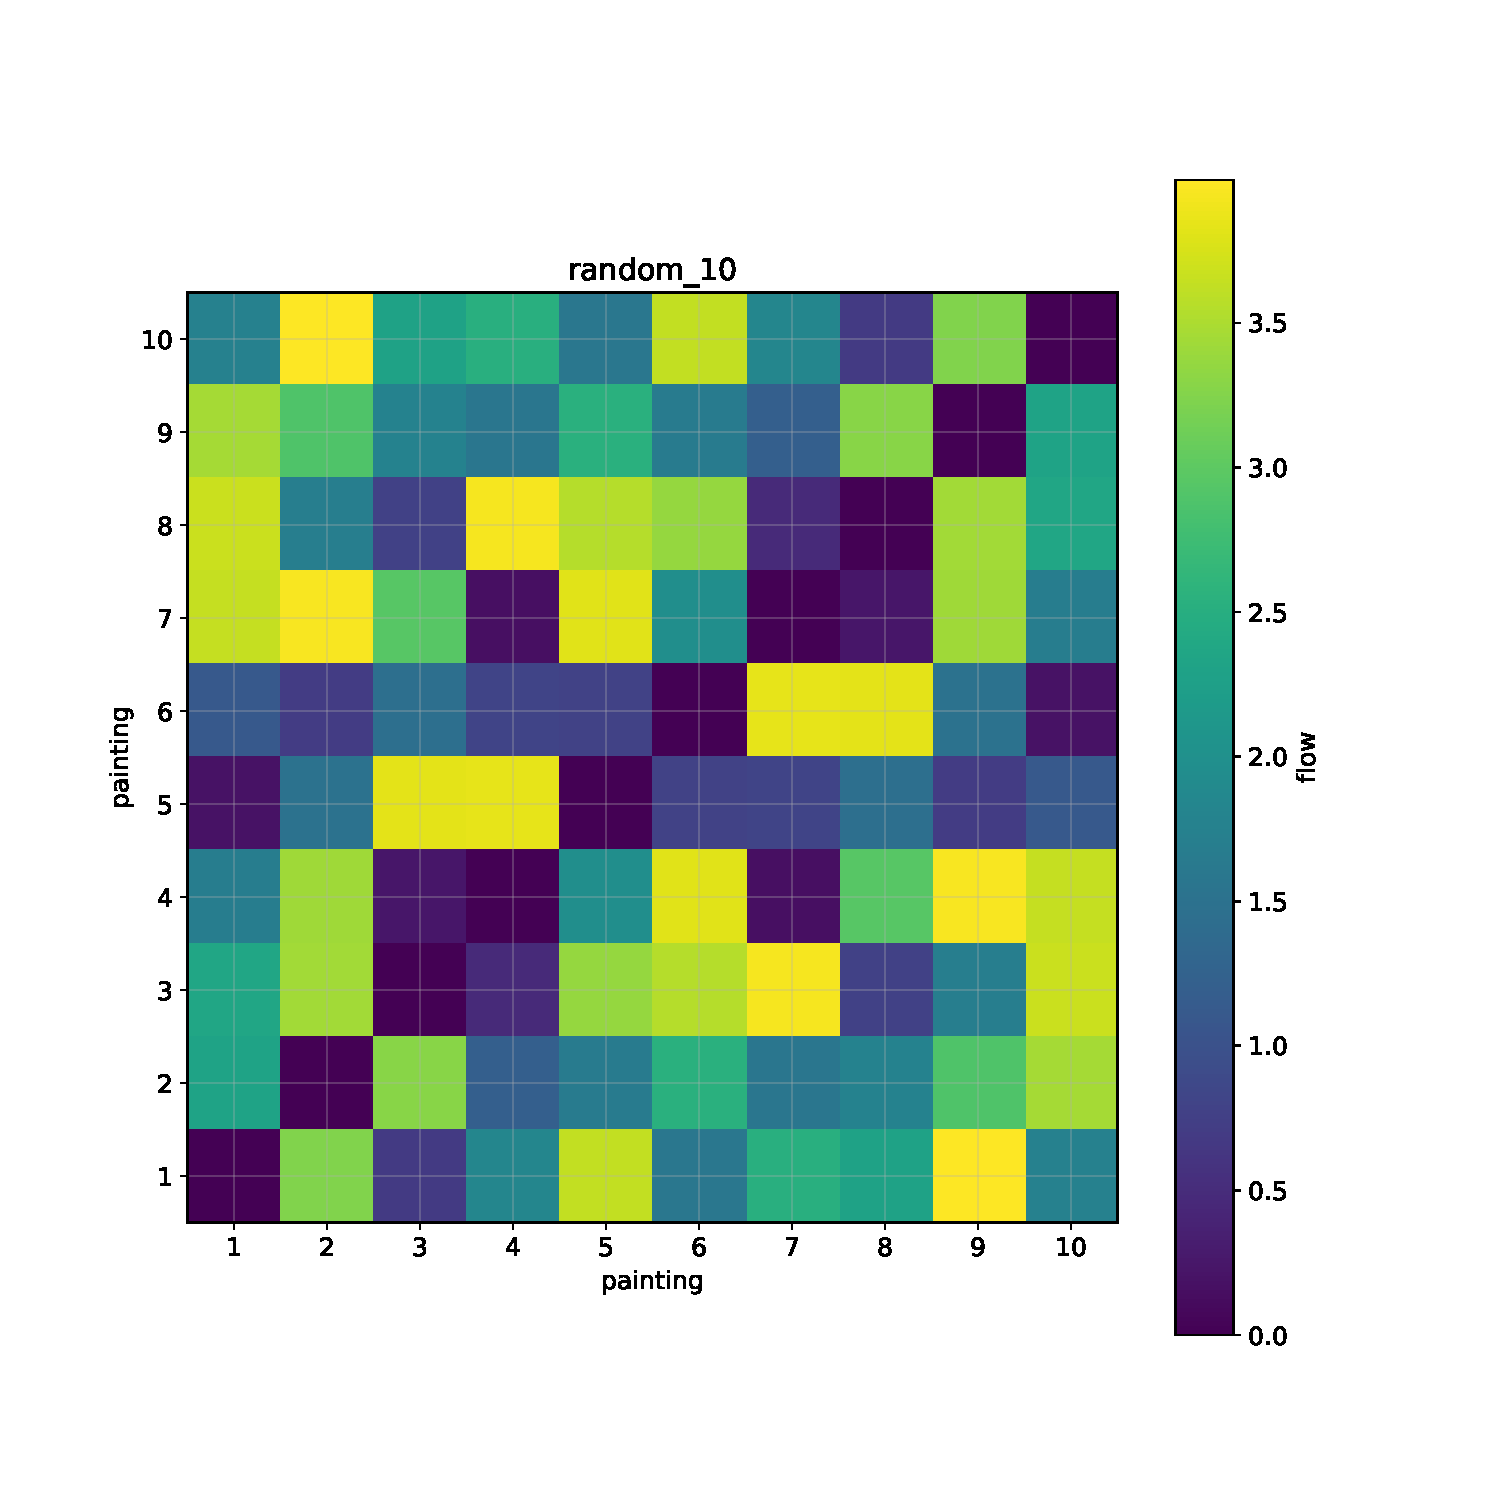
\includegraphics[width=0.8\textwidth]{heatmap_random_10}\label{subfig:heatmap-random-10}}
            \subfloat{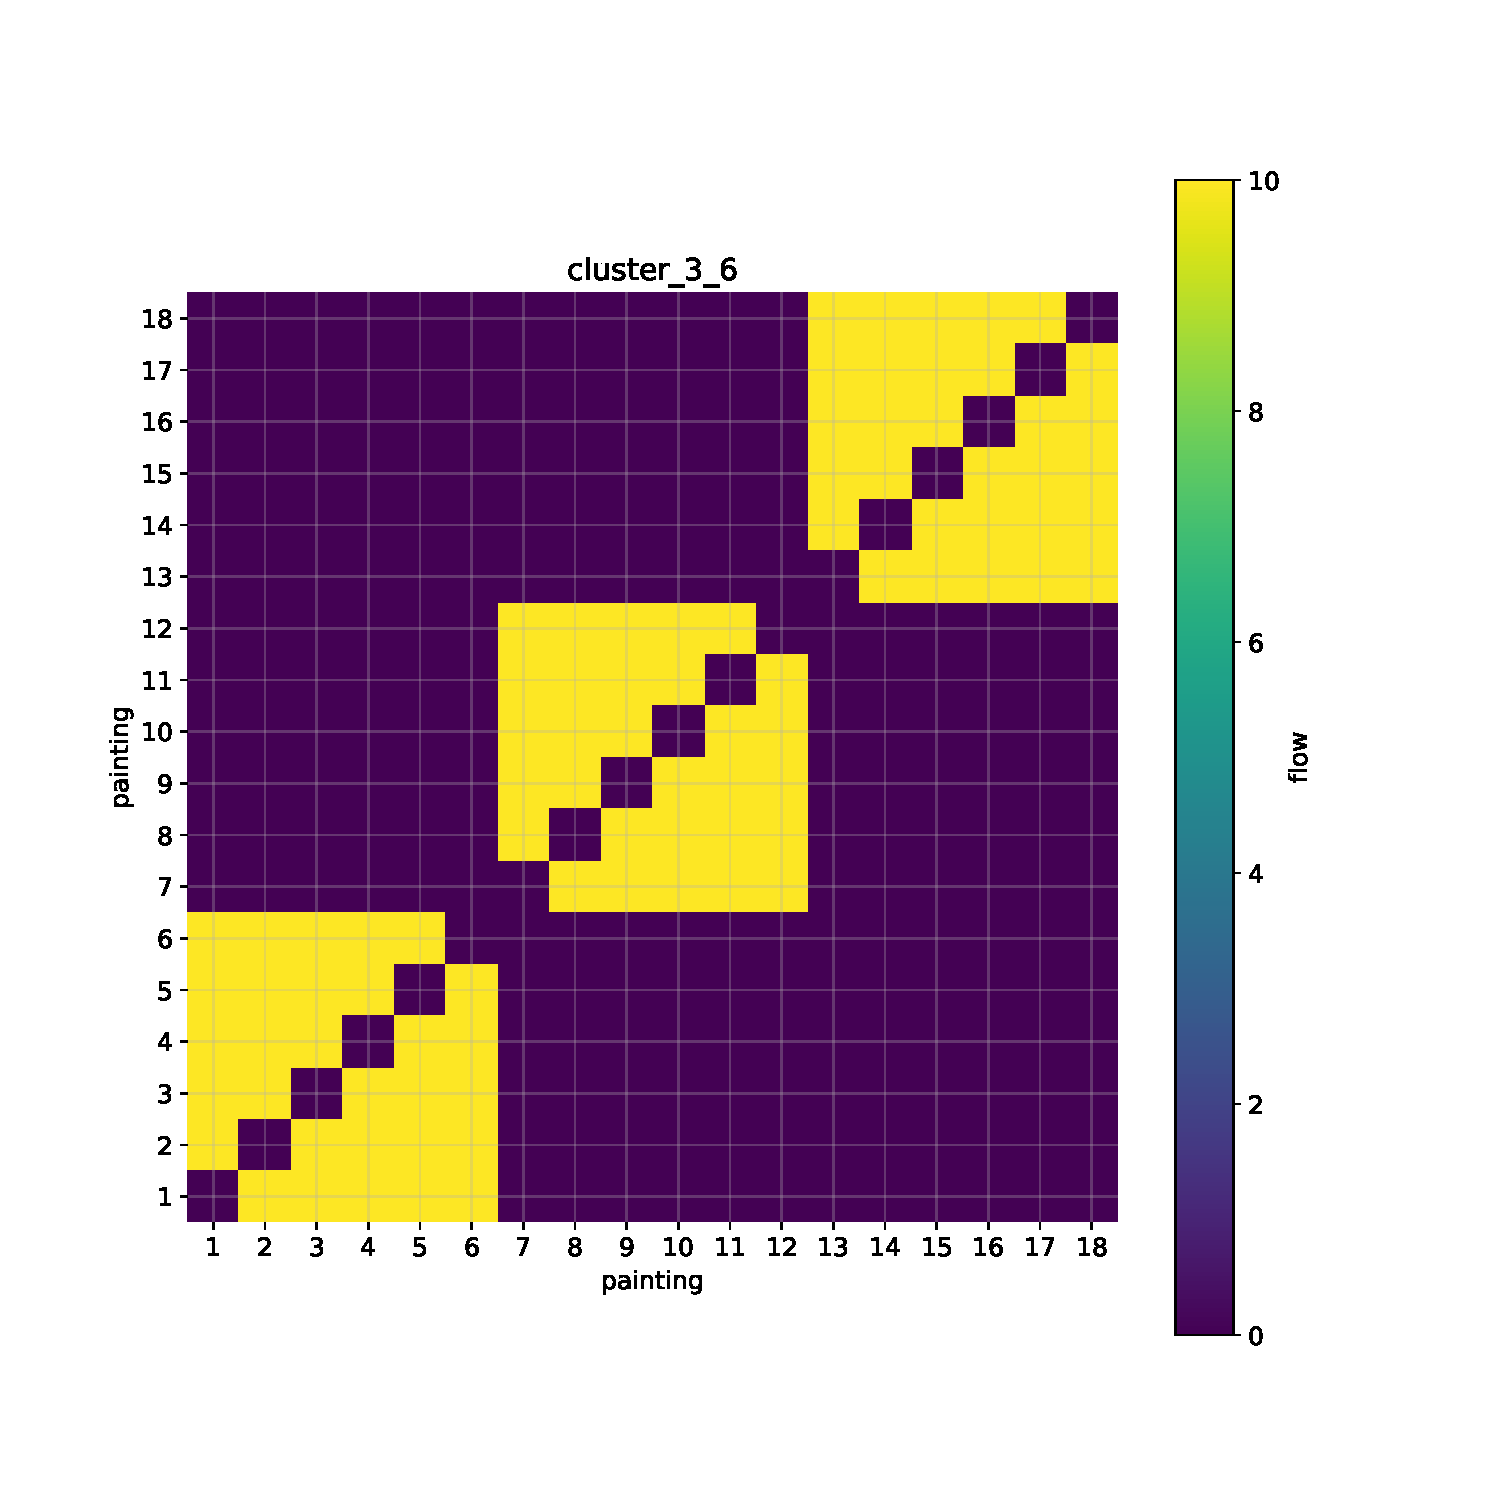
\includegraphics[width=0.8\textwidth]{heatmap_cluster_3_6}\label{subfig:heatmap-cluster-3-6}}
            \caption[Flow matrices examples]{Two flow matrices for random and clustering instances.
            Matrices are symmetric,i.e., the flow between two paintings is the same from each direction. Also, flow to/from itself is zero.}
            \label{fig:instance-flow}%
        \end{figure}
    \end{landscape}
    \clearpage% Flush page
}
